\section{Introduction}
\pagenumbering{arabic}
\subsection{Motivation}
Robot-based bin picking process automation offers enormous potential to completely transform bin picking tasks by boosting productivity, efficiency and cost-effectiveness. However, robot's capacity to adapt and learn from a variety of dynamic situations is the deciding factor in the success of bin picking applications. Transfer learning is a potent machine learning technique that could help with this problem by allowing robots to swiftly adapt to new tasks and situations by using the knowledge from pre-trained models \cite{danielthesis}. Transfer learning seeks to use information from one domain or task to enhance performance on a related domain or task. Conventional machine learning paradigms involve training models on a given dataset for a certain problem, starting from scratch. This involves a huge computational overhead and time and cost associated with it. But with transfer learning, even when the datasets or domains are distinct, the information obtained from one task can be helpful for completing a related task.

\vspace{5mm}

As the demand for efficient and cost effective machine learning solutions are on a rise in multiple sectors like robotic, computer vision, natural language processing and healthcare, more and more is the call for a source library in transfer learning. A handful number of reasons why a source library is necessary for transfer learning is elaborated below.
\begin{enumerate}
    \item \textbf{Faster Research and development} The entire pipeline for developing and testing a deep neural network from scratch can be intensely difficult and time-consuming. The process of research and development are sped up by the pool of tested models, datasets and algorithms that a source library provides.
    \item \textbf{Scalability to Diverse Domains} Transfer learning is used in numerous fields like robotics, time series analysis, image recognition and natural language processing. A source library provides frameworks that are adaptable to different tasks and datasets, as well as modular components that can be integrated with existing networks to be used in different applications.
    \item \textbf{Reproducibility and Accessibility} A collection of models, dataset and algorithms are available on using a source library in the transfer learning paradigm. Hence it facilitates cooperation, repeatability and transparency for researchers, developers and other stakeholders.
    \item \textbf{Minimization of Redundant Efforts} When developing similar algorithms or models, researchers frequently have to start from scratch in order to provide transfer learning solutions. A source library can reduce the effort in duplication of work and free up developers to work on new ideas and applications by offering pre-built components and reference implementations. Researchers can more efficiently compare results, assess performance and build upon each other's work by embracing standard frameworks, interfaces and evaluation criteria.
\end{enumerate}
Overall, a transfer learning source library fosters new research, increases access to state-of-the-art techniques and expedites the development of practical applications across a range of disciplines. Academics and researches are made possible by a centralized information repository and an ecology of collaboration using artificial intelligence and machine learning to tackle difficult challenges and find new opportunities for progress.

\subsection{Task and Goal}
Bin picking is fundamentally a pose estimation problem, which makes it a computer vision task. The solution to the bin picking problem is greatly influenced by the advancements in deep learning techniques for computer vision in recent years. At the moment, there are two available methods: model-free solutions and model-based ones. The model free methods rely on an image to find appropriate grasp poses, whereas the model-based solutions use \ac{CAD} models of items to detect them in a scene\cite{spenrath2022heuristic}. The bin picking application at \ac{IPA} utilizes an advanced model-based method initially based on PQ-Net++ from \cite{kleeberger2021precise}. The dataset used for this task is the ABC dataset\cite{Koch_2019_CVPR} which is a collection of one million \ac{CAD} models without any ground truth labels. It contains a large variety of objects, a handful of which are shown in Fig. \ref{fig:abc}.
\begin{figure}[t]
    \centering
    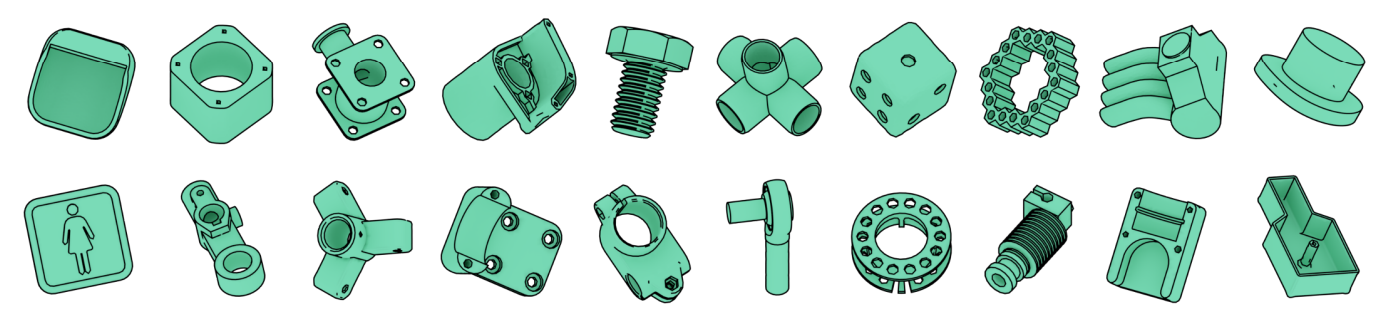
\includegraphics[width=350pt,height=150pt]{pictures/ABC.PNG}
    \caption{Some random objects from the ABC dataset.\cite{Koch_2019_CVPR}}
    \label{fig:abc}
  \end{figure}
\vspace{5mm}

The goal of this work is to develop a source library consisting of "good" source data which can be used as the data from the source domain in the further steps in a transfer learning pipeline. Therefore, the focus is to identify which features prevalent in an object makes it a "good" source data. A diverse collection of source data would be the objects that approximately captures the overall variance of the entire 1 million ABC dataset. Thus, it is trivial to think that more objects in the source library could better capture the overall variance of the dataset. But since the bin application is a model-based approach, it would be required to formulate the \ac{CAD} models of all these objects. Thus, having a large number of objects in the source library would entail high computational time for the generation of all the object models. Therefore, it is crucial to determine a permissible number of objects in the source library to facilitate its usage down the pipeline.  To further elaborate on this, if two objects are very similar to one-another than in spite of having a large similarity which just one other object, it loses the generalization capability of being nearly similar to a lot of other objects in the dataset. Hence, it would require a large amount of objects in the source library to capture the entire variance in the dataset. Thus, there is a trade-off between being very similar to a very small subset of objects and being approximately similar to a larger subset of objects in the dataset. Moreover, it is not universally defined which features in an object qualify as an important features and how it contributes in deciding whether an object is capable of becoming a viable source data. 
\subsection{Approach}
An end-to-end autoencoder proposed by \cite{mei2022unsupervised} is used to get the feature representations of the objects in the dataset\cite{Koch_2019_CVPR}. The autoencoder learns both the local and the global features of an object. Once the feature representation of the objects are obtained, they are grouped into clusters utilizing multiple clustering algorithm. A suitable clustering algorithm is utilized to get the representing members of the clusters. A high level overview of the entire method is shown in Fig. \ref{fig:overview}.
\begin{figure}[t]
  \centering
  \begin{tikzpicture}[node distance=2cm]        
      \node (autoencoder) [Autoencoder] {Autoencoder};
      \node (feat_rep) [Feat_Rep, right of=autoencoder, xshift=3cm] {Feature Representation};
      \node (clustering_algorithm) [Clustering_algorithm, below of=feat_rep, yshift=-0.5cm] {Clustering Algorithm};
      \node (rep_objs) [Rep_Objs, right of=clustering_algorithm, xshift=4cm] {Representative Objects};
      \draw [arrow] (autoencoder) -- (feat_rep);
      \draw [arrow] (feat_rep) -- (clustering_algorithm);  
      \draw [arrow] (clustering_algorithm) -- (rep_objs);       
  \end{tikzpicture}
  \caption{Overview of the entire pipeline for development of source library.}
  \label{fig:overview}
\end{figure}
 The clustering algorithm would not just consider the Euclidean distance between the datapoints but also other intrinsic features of the dataset such as the density because real world datasets are not necessarily globular in structure. A suitable evaluation metric such as \ac{DBCV}\cite{moulavi2014density} is used to compare the quality of the clustering algorithms which is robust to the size and shape of individual clusters as well as the outliers and noise of the dataset. Since, computing the \ac{DBCV} index on the entire dataset is extremely computationally expensive, the evaluation is performed on random batches of the subset. Moreover, the \ac{DBCV} is sensitive to the number of features in the dataset and fails to provide any tangible result in the presence of a large number of features (e.g. over 150). Thus, a dimensionality reduction is necessary for the evaluation of the clustering algorithm. Once, the clustering algorithm with best results in the evaluation metrics is achieved the entire dataset is categorized into a number of clusters, where the medoid of the cluster is chosen as the representative member of the cluster. The similarity of the test dataset with the representative members of the datasets shows the generalization quality of the source library. The approximate time for each step of the work is shown in Tab. \ref{tab:overview_time}.

\begin{table}[ht]
  \caption{Overview of the approximate time taken for the creation of the source library}
  \label{tab:overview_time}
  \centering
  \begin{tabular}{|l|l|}
    \toprule
    Step & Time \\
    \midrule
    Training the model & 28 hours\\
    Dimensionality reduction & 4 hours \\        
    Clustering Algorithm & 3 hours \\
    Similarity evaluation & 11 minutes\\
    \bottomrule
  \end{tabular}
\end{table}
\subsection{Contribution}
Although density-based clustering algorithm like \ac{DBSCAN} and \ac{HDBSCAN} shows promising results when the clusters in real-world datasets aren't globular in nature, yet the current existing implementations in the literature doesn't put any restrictions on the number of clusters returned by the clusters. In case of very large datasets like the ABC dataset\cite{Koch_2019_CVPR}, these algorithms return a large number of clusters (over multiple thousands). The model generation of such thousands of objects aren't feasible or efficient in business situations such as in \ac{IPA}. Thus, novel contribution in this work is stated as follows:
\begin{itemize}
  \item The idea of multi-level \ac{HDBSCAN} algorithm is proposed in this work to limit the number of clusters to a feasible number but also retain the properties of a density based clustering algorithm.
  \item An extensive experimentation on the optimal hyperparameter values during model training has been carried on for the development of a high performing network used for the generation of feature representations of the objects in the dataset.
\end{itemize}
\cleardoublepage